\documentclass[12pt]{standalone}
\usepackage{amssymb} % мат. символы
    \DeclareMathSymbol{\sm}{\mathbin}{AMSa}{"39} % короткий минус
    \newcommand{\mo}{\sm\!1}
\usepackage{bm}
    \newcommand{\bma}{{\bm{\alpha}}}
    \newcommand{\bmb}{{\bm{\beta}}}
    
\usepackage{tikz}
    \usetikzlibrary{arrows.meta}
    \usetikzlibrary{calc}
\tikzset{gdst/.style=
    {circle, draw=black!60, very thick, minimum height=1.2cm, inner sep=2pt, text centered, }, }

\begin{document}
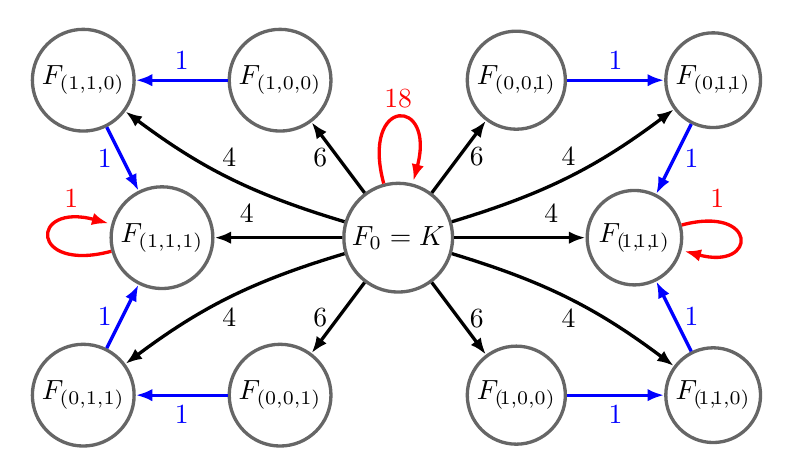
\begin{tikzpicture}
    \node[gdst] (f0)  at (0,0)     {$F_{0}=K$};
    \node[gdst] (f1)  at (-1.5,-2) {$F_{(0,0,1)}$};
    \node[gdst] (f2)  at (1.5,-2)  {$F_{(\mo,0,0)}$};
    \node[gdst] (f3)  at (1.5,2)   {$F_{(0,0,\mo)}$};
    \node[gdst] (f4)  at (-1.5,2)  {$F_{(1,0,0)}$};
    \node[gdst] (f5)  at (-4,-2)   {$F_{(0,1,1)}$};
    \node[gdst] (f6)  at (4,-2)    {$F_{(\mo,\mo,0)}$};
    \node[gdst] (f7)  at (4,2)     {$F_{(0,\mo,\mo)}$};
    \node[gdst] (f8)  at (-4,2)    {$F_{(1,1,0)}$};
    \node[gdst] (f9)  at (-3,0)    {$F_{(1,1,1)}$};
    \node[gdst] (f10) at (3,0)     {$F_{(\mo,\mo,\mo)}$};
    \path[->,>={Latex[length=6pt]}, very thick] 
        (f0)edge[loop above, red] node[above] {18} (f0)
            edge node[left] {6} (f1)
            edge node[right] {6} (f2)
            edge node[right] {6} (f3)
            edge node[left] {6} (f4)
            edge[bend right=10] node[below] {4} (f5)
            edge[bend left=10] node[below] {4} (f6)
            edge[bend right=10] node[above] {4} (f7)
            edge[bend left=10] node[above] {4} (f8)
            edge node[shift={(-0.4,0.3)}] {4} (f9)
            edge node[shift={(0.4,0.3)}] {4} (f10)
        (f1)edge[blue] node[below] {1} (f5)
        (f2)edge[blue] node[below] {1} (f6)
        (f3)edge[blue] node[above] {1} (f7)
        (f4)edge[blue] node[above] {1} (f8)
        (f5)edge[blue] node[left] {1} (f9)
        (f6)edge[blue] node[right] {1} (f10)
        (f7)edge[blue] node[right] {1} (f10)
        (f8)edge[blue] node[left] {1} (f9)
        (f9)edge[loop left, red] node[shift={(0.5,0.5)}] {1} (f9)
        (f10)edge[loop right, red] node[shift={(-0.5,0.5)}] {1} (f10)
        ;
\end{tikzpicture}
\qquad\qquad
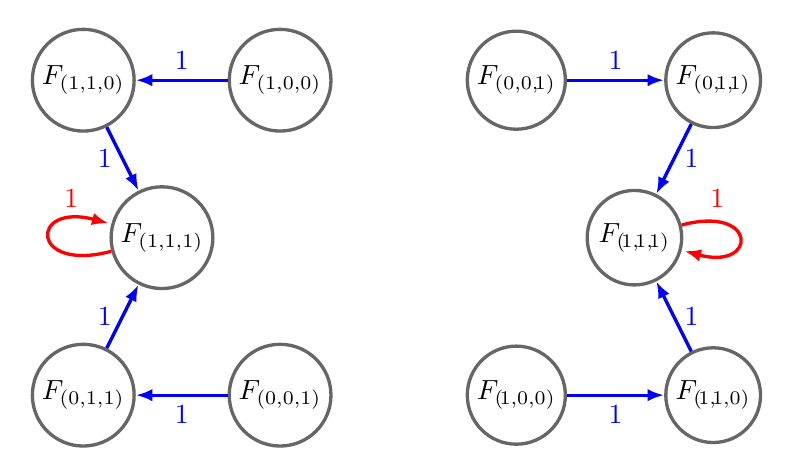
\begin{tikzpicture}
    \node[gdst] (f1)  at (-1.5,-2) {$F_{(0,0,1)}$};
    \node[gdst] (f2)  at (1.5,-2)  {$F_{(\mo,0,0)}$};
    \node[gdst] (f3)  at (1.5,2)   {$F_{(0,0,\mo)}$};
    \node[gdst] (f4)  at (-1.5,2)  {$F_{(1,0,0)}$};
    \node[gdst] (f5)  at (-4,-2)   {$F_{(0,1,1)}$};
    \node[gdst] (f6)  at (4,-2)    {$F_{(\mo,\mo,0)}$};
    \node[gdst] (f7)  at (4,2)     {$F_{(0,\mo,\mo)}$};
    \node[gdst] (f8)  at (-4,2)    {$F_{(1,1,0)}$};
    \node[gdst] (f9)  at (-3,0)    {$F_{(1,1,1)}$};
    \node[gdst] (f10) at (3,0)     {$F_{(\mo,\mo,\mo)}$};
    \path[->,>={Latex[length=6pt]}, very thick] 
        (f1)edge[blue] node[below] {1} (f5)
        (f2)edge[blue] node[below] {1} (f6)
        (f3)edge[blue] node[above] {1} (f7)
        (f4)edge[blue] node[above] {1} (f8)
        (f5)edge[blue] node[left] {1} (f9)
        (f6)edge[blue] node[right] {1} (f10)
        (f7)edge[blue] node[right] {1} (f10)
        (f8)edge[blue] node[left] {1} (f9)
        (f9)edge[loop left, red] node[shift={(0.5,0.5)}] {1} (f9)
        (f10)edge[loop right, red] node[shift={(-0.5,0.5)}] {1} (f10)
        ;
\end{tikzpicture}
\end{document}